\subsubsection{Caso d'uso UC8.1.3.2: Creazione domanda a risposta multipla}
	\label{UC8.1.3.2}
	\begin{figure}[h]
		\centering
			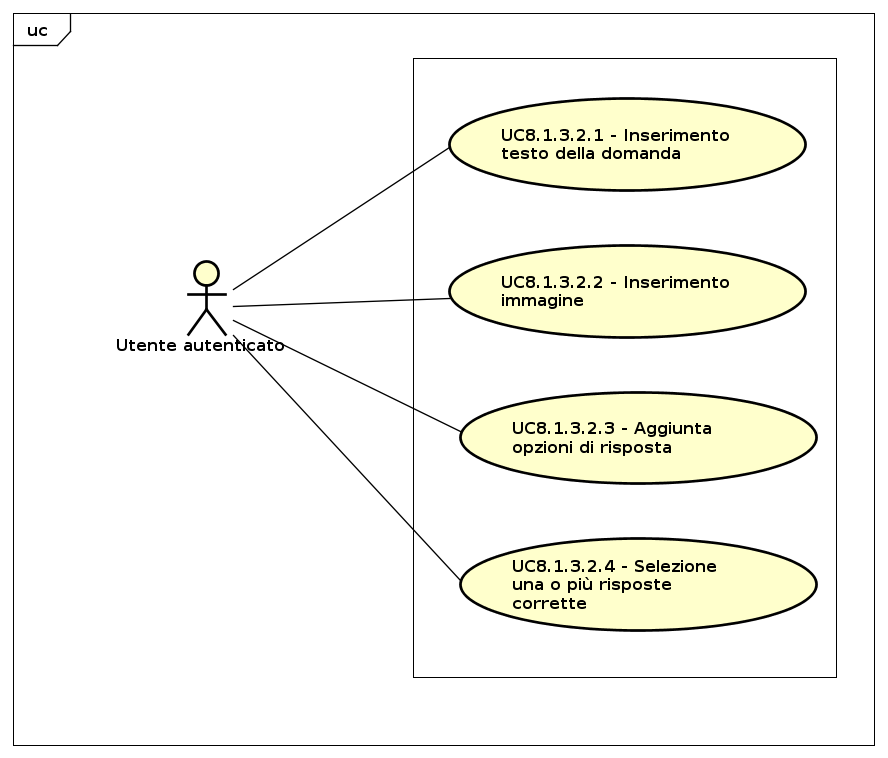
\includegraphics[scale=0.45,keepaspectratio]{UML/UC8_1_3_2.png}
		\caption{UC8.1.3.2: Creazione domanda a risposta multipla}
	\end{figure}
	\FloatBarrier
	\begin{itemize}
		\item
			\textbf{Attori}: utente autenticato, utente autenticato pro;
		\item		
			\textbf{Descrizione}: lo scopo di questa funzionalità è offrire agli attori la possibilità di creare domande a risposta multipla;
		\item
			\textbf{Precondizione}: gli attori hanno selezionato la seguente funzionalità; 
		\item
			\textbf{Postcondizione}: gli attori hanno creato una domanda a risposta multipla;
		\item
			\textbf{Scenario principale}:
	       		\begin{enumerate}
	       			\item
	       			Gli attori devono compilare il campo dati destinato alla scrittura del testo della domanda (UC8.1.3.2.1)
	       			\item
	       			Gli attori possono inserire un'immagine relativa al testo della domanda (UC8.1.3.2.2)
	       			\item
	       			Gli attori devono aggiungere almeno due opzioni di risposta (UC8.1.3.2.3);
					\item
					Gli attori devono indicare una o più risposte corrette (UC8.1.3.2.4).
	 			\end{enumerate}
	\end{itemize}

\subsubsection{Caso d'uso UC8.1.3.2.1: Inserimento testo della domanda}
	\begin{itemize}
		\item
			\textbf{Attori}: utente autenticato, utente autenticato pro;
		\item		
			\textbf{Descrizione}: lo scopo di questa funzionalità è offrire agli attori la possibilità di inserire il testo della domanda;
		\item
			\textbf{Precondizione}: gli attori hanno selezionato la funzionalità di creazione di una domanda a risposta multipla; 
		\item
			\textbf{Postcondizione}: gli attori hanno inserito il testo della domanda;
		\item
			\textbf{Scenario principale}: gli attori inseriscono il testo della domanda. 
	 			
	\end{itemize}
	
\subsubsection{Caso d'uso UC8.1.3.2.2: Inserimento immagine}
	\begin{itemize}
		\item
			\textbf{Attori}: utente autenticato, utente autenticato pro;
		\item		
			\textbf{Descrizione}: lo scopo di questa funzionalità è offrire agli attori la possibilità di inserire un'immagine relativa al testo della domanda;
		\item
			\textbf{Precondizione}: gli attori hanno selezionato la funzionalità di creazione di una domanda a risposta multipla; 
		\item
			\textbf{Postcondizione}: gli attori hanno inserito l'immagine;
		\item
			\textbf{Scenario principale}: gli attori inseriscono l'immagine. 	
	\end{itemize}
	
	
\subsubsection{Caso d'uso UC8.1.3.2.3: Aggiunta opzioni di risposta}
	\begin{itemize}
		\item
			\textbf{Attori}: utente autenticato, utente autenticato pro;
		\item		
			\textbf{Descrizione}: lo scopo di questa funzionalità è offrire agli attori la possibilità di aggiungere almeno due opzioni di risposta;
		\item
			\textbf{Precondizione}: gli attori hanno selezionato la funzionalità di creazione di una domanda a risposta multipla; 
		\item
			\textbf{Postcondizione}: gli attori hanno aggiunto due o più opzioni di risposta;
		\item
			\textbf{Scenario principale}:
	       		\begin{enumerate}
	       			\item
	       			Gli attori possono aggiungere opzioni di risposta che includono testo (UC8.1.3.2.3.1);
					\item
					Gli attori possono aggiungere opzioni di risposta che includono immagini (UC8.1.3.2.3.2).
	 			\end{enumerate}
	\end{itemize}	
	
\subsubsection{Caso d'uso UC8.1.3.2.3.1: Aggiunta opzioni di risposta che includono testo}
	\begin{itemize}
		\item
			\textbf{Attori}: utente autenticato, utente autenticato pro;
		\item		
			\textbf{Descrizione}: lo scopo di questa funzionalità è offrire agli attori la possibilità di aggiungere almeno due opzioni di risposta che includono testo;
		\item
			\textbf{Precondizione}: gli attori hanno selezionato la funzionalità di creazione di domande a risposta multipla con opzioni di risposta che includono testo; 
		\item
			\textbf{Postcondizione}: gli attori hanno aggiunto due o più opzioni di risposta che includono testo;
		\item
			\textbf{Scenario principale}: gli attori aggiungono due o più opzioni di risposta che includono testo. 			
	\end{itemize}	
	
\subsubsection{Caso d'uso UC8.1.3.2.3.2: Aggiunta opzioni di risposta che includono immagini}
	\begin{itemize}
		\item
			\textbf{Attori}: utente autenticato, utente autenticato pro;
		\item		
			\textbf{Descrizione}: lo scopo di questa funzionalità è offrire agli attori la possibilità di aggiungere almeno due opzioni di risposta che includono immagini;
		\item
			\textbf{Precondizione}: gli attori hanno selezionato la funzionalità di creazione di domande a risposte multipla con opzioni di risposta che includono immagini; 
		\item
			\textbf{Postcondizione}: gli attori hanno aggiunto due o più opzioni di risposta che includono immagini;
		\item
			\textbf{Scenario principale}: gli attori aggiungono due o più opzioni di risposta che includono immagini. 			
	\end{itemize}
	
\subsubsection{Caso d'uso UC8.1.3.2.4: Selezione una o più risposte corrette}
	\begin{itemize}
		\item
			\textbf{Attori}: utente autenticato, utente autenticato pro;
		\item		
			\textbf{Descrizione}: lo scopo di questa funzionalità è offrire agli attori la possibilità di selezionare una o più risposte corrette;
		\item
			\textbf{Precondizione}: gli attori hanno selezionato la funzionalità di creazione di domande a risposta multipla; 
		\item
			\textbf{Postcondizione}: gli attori hanno selezionato una o più risposte corrette;
		\item
			\textbf{Scenario principale}: gli attori selezionano una o più risposte corrette. 			
	\end{itemize}

	
	
	
	
	
	
	